% $Header: /u/gcmpack/manual/s_algorithm/text/time_stepping.tex,v 1.8 2001/10/05 19:41:08 adcroft Exp $
% $Name:  $

The equations of motion integrated by the model involve four
prognostic equations for flow, $u$ and $v$, temperature, $\theta$, and
salt/moisture, $S$, and three diagnostic equations for vertical flow,
$w$, density/buoyancy, $\rho$/$b$, and pressure/geo-potential,
$\phi_{hyd}$. In addition, the surface pressure or height may by
described by either a prognostic or diagnostic equation and if
non-hydrostatics terms are included then a diagnostic equation for
non-hydrostatic pressure is also solved. The combination of prognostic
and diagnostic equations requires a model algorithm that can march
forward prognostic variables while satisfying constraints imposed by
diagnostic equations.

Since the model comes in several flavours and formulation, it would be
confusing to present the model algorithm exactly as written into code
along with all the switches and optional terms. Instead, we present
the algorithm for each of the basic formulations which are:
\begin{enumerate}
\item the semi-implicit pressure method for hydrostatic equations
with a rigid-lid, variables co-located in time and with
Adams-Bashforth time-stepping, \label{it:a}
\item as \ref{it:a}. but with an implicit linear free-surface, \label{it:b}
\item as \ref{it:a}. or \ref{it:b}. but with variables staggered in time,
\label{it:c}
\item as \ref{it:a}. or \ref{it:b}. but with non-hydrostatic terms included,
\item as \ref{it:b}. or \ref{it:c}. but with non-linear free-surface.
\end{enumerate}

In all the above configurations it is also possible to substitute the
Adams-Bashforth with an alternative time-stepping scheme for terms
evaluated explicitly in time. Since the over-arching algorithm is
independent of the particular time-stepping scheme chosen we will
describe first the over-arching algorithm, known as the pressure
method, with a rigid-lid model in section
\ref{sect:pressure-method-rigid-lid}. This algorithm is essentially
unchanged, apart for some coefficients, when the rigid lid assumption
is replaced with a linearized implicit free-surface, described in
section \ref{sect:pressure-method-linear-backward}. These two flavours
of the pressure-method encompass all formulations of the model as it
exists today. The integration of explicit in time terms is out-lined
in section \ref{sect:adams-bashforth} and put into the context of the
overall algorithm in sections \ref{sect:adams-bashforth-sync} and
\ref{sect:adams-bashforth-staggered}. Inclusion of non-hydrostatic
terms requires applying the pressure method in three dimensions
instead of two and this algorithm modification is described in section
\ref{sect:non-hydrostatic}. Finally, the free-surface equation may be
treated more exactly, including non-linear terms, and this is
described in section \ref{sect:nonlinear-freesurface}.


\section{Pressure method with rigid-lid} \label{sect:pressure-method-rigid-lid}

\begin{figure}
\begin{center}
\resizebox{4.0in}{!}{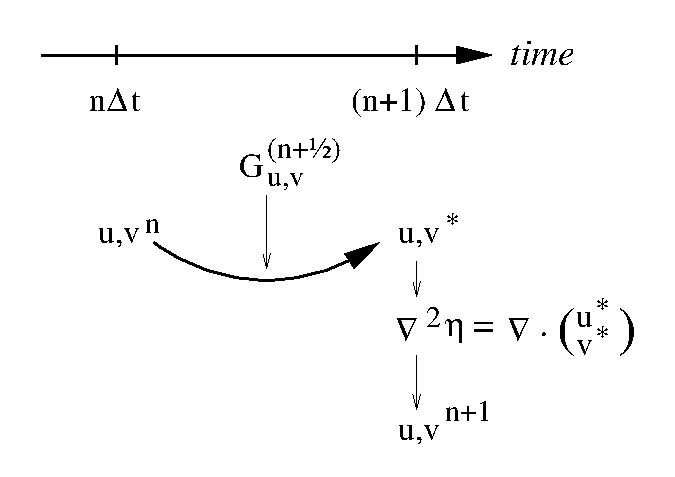
\includegraphics{part2/pressure-method-rigid-lid.eps}}
\end{center}
\caption{
A schematic of the evolution in time of the pressure method
algorithm. A prediction for the flow variables at time level $n+1$ is
made based only on the explicit terms, $G^{(n+^1/_2)}$, and denoted
$u^*$, $v^*$. Next, a pressure field is found such that $u^{n+1}$,
$v^{n+1}$ will be non-divergent. Conceptually, the $*$ quantitites
exist at time level $n+1$ but they are intermediate and only
temporary.}
\label{fig:pressure-method-rigid-lid}
\end{figure}

\begin{figure}
\begin{center} \fbox{ \begin{minipage}{4.5in} \begin{tabbing}
aaa \= aaa \= aaa \= aaa \= aaa \= aaa \kill 
FORWARD\_STEP \\
\> DYNAMICS \\
\>\> TIMESTEP \` $u^*$,$v^*$ (\ref{eq:ustar-rigid-lid},\ref{eq:vstar-rigid-lid}) \\
\> SOLVE\_FOR\_PRESSURE \\
\>\> CALC\_DIV\_GHAT \` $H\widehat{u^*}$,$H\widehat{v^*}$ (\ref{eq:elliptic}) \\
\>\> CG2D \` $\eta^{n+1}$ (\ref{eq:elliptic}) \\
\> THE\_CORRECTION\_STEP  \\
\>\> CALC\_GRAD\_PHI\_SURF \` $\nabla \eta^{n+1}$ \\
\>\> CORRECTION\_STEP \` $u^{n+1}$,$v^{n+1}$ (\ref{eq:un+1-rigid-lid},\ref{eq:vn+1-rigid-lid})
\end{tabbing} \end{minipage} } \end{center}
\caption{Calling tree for the pressure method alogtihm}
\label{fig:call-tree-pressure-method}
\end{figure}

The horizontal momentum and continuity equations for the ocean
(\ref{eq:ocean-mom} and \ref{eq:ocean-cont}), or for the atmosphere
(\ref{eq:atmos-mom} and \ref{eq:atmos-cont}), can be summarized by:
\begin{eqnarray}
\partial_t u + g \partial_x \eta & = & G_u \\
\partial_t v + g \partial_y \eta & = & G_v \\
\partial_x u + \partial_y v + \partial_z w & = & 0
\end{eqnarray}
where we are adopting the oceanic notation for brevity. All terms in
the momentum equations, except for surface pressure gradient, are
encapsulated in the $G$ vector. The continuity equation, when
integrated over the fluid depth, $H$, and with the rigid-lid/no normal
flow boundary conditions applied, becomes:
\begin{equation}
\partial_x H \widehat{u} + \partial_y H \widehat{v} = 0
\label{eq:rigid-lid-continuity}
\end{equation}
Here, $H\widehat{u} = \int_H u dz$ is the depth integral of $u$,
similarly for $H\widehat{v}$. The rigid-lid approzimation sets $w=0$
at the lid so that it does not move but allows a pressure to be
exerted on the fluid by the lid. The horizontal momentum equations and
vertically integrated continuity equation are be discretized in time
and space as follows:
\begin{eqnarray}
u^{n+1} + \Delta t g \partial_x \eta^{n+1}
& = & u^{n} + \Delta t G_u^{(n+1/2)}
\label{eq:discrete-time-u}
\\
v^{n+1} + \Delta t g \partial_y \eta^{n+1}
& = & v^{n} + \Delta t G_v^{(n+1/2)}
\label{eq:discrete-time-v}
\\
  \partial_x H \widehat{u^{n+1}}
+ \partial_y H \widehat{v^{n+1}} & = & 0
\label{eq:discrete-time-cont-rigid-lid}
\end{eqnarray}
As written here, terms on the LHS all involve time level $n+1$ and are
referred to as implicit; the implicit backward time stepping scheme is
being used. All other terms in the RHS are explicit in time. The
thermodynamic quantities are integrated forward in time in parallel
with the flow and will be discussed later. For the purposes of
describing the pressure method it suffices to say that the hydrostatic
pressure gradient is explicit and so can be included in the vector
$G$.

Substituting the two momentum equations into the depth integrated
continuity equation eliminates $u^{n+1}$ and $v^{n+1}$ yeilding an
elliptic equation for $\eta^{n+1}$. Equations
\ref{eq:discrete-time-u}, \ref{eq:discrete-time-v} and
\ref{eq:discrete-time-cont-rigid-lid} can then be re-arranged as follows:
\begin{eqnarray}
u^{*} & = & u^{n} + \Delta t G_u^{(n+1/2)} \label{eq:ustar-rigid-lid} \\
v^{*} & = & v^{n} + \Delta t G_v^{(n+1/2)} \label{eq:vstar-rigid-lid} \\
  \partial_x \Delta t g H \partial_x \eta^{n+1}
+ \partial_y \Delta t g H \partial_y \eta^{n+1}
& = &
  \partial_x H \widehat{u^{*}}
+ \partial_y H \widehat{v^{*}} \label{eq:elliptic}
\\
u^{n+1} & = & u^{*} - \Delta t g \partial_x \eta^{n+1} \label{eq:un+1-rigid-lid}\\
v^{n+1} & = & v^{*} - \Delta t g \partial_y \eta^{n+1} \label{eq:vn+1-rigid-lid}
\end{eqnarray}
Equations \ref{eq:ustar-rigid-lid} to \ref{eq:vn+1-rigid-lid}, solved
sequentially, represent the pressure method algorithm used in the
model. The essence of the pressure method lies in the fact that any
explicit prediction for the flow would lead to a divergence flow field
so a pressure field must be found that keeps the flow non-divergent
over each step of the integration. The particular location in time of
the pressure field is somewhat ambiguous; in
Fig.~\ref{fig:pressure-method-rigid-lid} we depicted as co-located
with the future flow field (time level $n+1$) but it could equally
have been drawn as staggered in time with the flow.

The correspondance to the code is as follows:
\begin{itemize}
\item
the prognostic phase, equations \ref{eq:ustar-rigid-lid} and \ref{eq:vstar-rigid-lid},
stepping forward $u^n$ and $v^n$ to $u^{*}$ and $v^{*}$ is coded in
{\em TIMESTEP.F}
\item
the vertical integration, $H \widehat{u^*}$ and $H
\widehat{v^*}$, divergence and invertion of the elliptic operator in
equation \ref{eq:elliptic} is coded in {\em
SOLVE\_FOR\_PRESSURE.F}
\item
finally, the new flow field at time level $n+1$ given by equations
\ref{eq:un+1-rigid-lid} and \ref{eq:vn+1-rigid-lid} is calculated in {\em CORRECTION\_STEP.F}.
\end{itemize}
The calling tree for these routines is given in
Fig.~\ref{fig:call-tree-pressure-method}.



\paragraph{Need to discuss implicit viscosity somewhere:}
\begin{eqnarray}
\frac{1}{\Delta t} u^{n+1} - \partial_z A_v \partial_z u^{n+1}
+ g \partial_x \eta^{n+1} & = & \frac{1}{\Delta t} u^{n} +
G_u^{(n+1/2)}
\\
\frac{1}{\Delta t} v^{n+1} - \partial_z A_v \partial_z v^{n+1}
+ g \partial_y \eta^{n+1} & = & \frac{1}{\Delta t} v^{n} + G_v^{(n+1/2)}
\end{eqnarray}


\section{Pressure method with implicit linear free-surface}
\label{sect:pressure-method-linear-backward}

The rigid-lid approximation filters out external gravity waves
subsequently modifying the dispersion relation of barotropic Rossby
waves. The discrete form of the elliptic equation has some zero
eigen-values which makes it a potentially tricky or inefficient
problem to solve.

The rigid-lid approximation can be easily replaced by a linearization
of the free-surface equation which can be written:
\begin{equation}
\partial_t \eta + \partial_x H \widehat{u} + \partial_y H \widehat{v} = P-E+R
\label{eq:linear-free-surface=P-E+R}
\end{equation}
which differs from the depth integrated continuity equation with
rigid-lid (\ref{eq:rigid-lid-continuity}) by the time-dependent term
and fresh-water source term.

Equation \ref{eq:discrete-time-cont-rigid-lid} in the rigid-lid
pressure method is then replaced by the time discretization of
\ref{eq:linear-free-surface=P-E+R} which is:
\begin{equation}
\eta^{n+1}
+ \Delta t \partial_x H \widehat{u^{n+1}}
+ \Delta t \partial_y H \widehat{v^{n+1}}
=
\eta^{n}
+ \Delta t ( P - E + R )
\label{eq:discrete-time-backward-free-surface}
\end{equation}
where the use of flow at time level $n+1$ makes the method implicit
and backward in time. The is the preferred scheme since it still
filters the fast unresolved wave motions by damping them. A centered
scheme, such as Crank-Nicholson, would alias the energy of the fast
modes onto slower modes of motion.

As for the rigid-lid pressure method, equations
\ref{eq:discrete-time-u}, \ref{eq:discrete-time-v} and
\ref{eq:discrete-time-backward-free-surface} can be re-arranged as follows:
\begin{eqnarray}
u^{*} & = & u^{n} + \Delta t G_u^{(n+1/2)} \label{eq:ustar-backward-free-surface} \\
v^{*} & = & v^{n} + \Delta t G_v^{(n+1/2)} \label{eq:vstar-backward-free-surface} \\
\eta^* & = & \epsilon_{fs} \left( \eta^{n} +P-E+R \right)- \Delta t 
  \partial_x H \widehat{u^{*}}
+ \partial_y H \widehat{v^{*}}
\\
  \partial_x g H \partial_x \eta^{n+1}
+ \partial_y g H \partial_y \eta^{n+1}
- \frac{\epsilon_{fs} \eta^{n+1}}{\Delta t^2}
& = &
- \frac{\eta^*}{\Delta t^2}
\label{eq:elliptic-backward-free-surface}
\\
u^{n+1} & = & u^{*} - \Delta t g \partial_x \eta^{n+1} \label{eq:un+1-backward-free-surface}\\
v^{n+1} & = & v^{*} - \Delta t g \partial_y \eta^{n+1} \label{eq:vn+1-backward-free-surface}
\end{eqnarray}
Equations~\ref{eq:ustar-backward-free-surface}
to~\ref{eq:vn+1-backward-free-surface}, solved sequentially, represent
the pressure method algorithm with a backward implicit, linearized
free surface. The method is still formerly a pressure method because
in the limit of large $\Delta t$ the rigid-lid method is
reovered. However, the implicit treatment of the free-surface allows
the flow to be divergent and for the surface pressure/elevation to
respond on a finite time-scale (as opposed to instantly). To recovere
the rigid-lid formulation, we introduced a switch-like parameter,
$\epsilon_{fs}$, which selects between the free-surface and rigid-lid;
$\epsilon_{fs}=1$ allows the free-surface to evolve; $\epsilon_{fs}=0$
imposes the rigid-lid. The evolution in time and location of variables
is exactly as it was for the rigid-lid model so that
Fig.~\ref{fig:pressure-method-rigid-lid} is still
applicable. Similarly, the calling sequence, given in
Fig.~\ref{fig:call-tree-pressure-method}, is as for the
pressure-method.


\section{Explicit time-stepping: Adams-Bashforth}
\label{sect:adams-bashforth}

In describing the the pressure method above we deferred describing the
time discretization of the explicit terms. We have historically used
the quasi-second order Adams-Bashforth method for all explicit terms
in both the momentum and tracer equations. This is still the default
mode of operation but it is now possible to use alternate schemes for
tracers (see section \ref{sect:tracer-advection}).

\begin{figure}
\begin{center} \fbox{ \begin{minipage}{4.5in} \begin{tabbing}
aaa \= aaa \= aaa \= aaa \= aaa \= aaa \kill 
FORWARD\_STEP \\
\> THERMODYNAMICS \\
\>\> CALC\_GT \\
\>\>\> GAD\_CALC\_RHS \` $G_\theta^n = G_\theta( u, \theta^n )$ \\
\>\>\> EXTERNAL\_FORCING \` $G_\theta^n = G_\theta^n + {\cal Q}$ \\
\>\>\> ADAMS\_BASHFORTH2 \` $G_\theta^{(n+1/2)}$ (\ref{eq:adams-bashforth2}) \\
\>\> TIMESTEP\_TRACER \` $\tau^*$ (\ref{eq:taustar}) \\
\>\> IMPLDIFF \` $\tau^{(n+1)}$ (\ref{eq:tau-n+1-implicit})
\end{tabbing} \end{minipage} } \end{center}
\caption{
Calling tree for the Adams-Bashforth time-stepping of temperature with
implicit diffusion.}
\label{fig:call-tree-adams-bashforth}
\end{figure}

In the previous sections, we summarized an explicit scheme as:
\begin{equation}
\tau^{*} = \tau^{n} + \Delta t G_\tau^{(n+1/2)}
\label{eq:taustar}
\end{equation}
where $\tau$ could be any prognostic variable ($u$, $v$, $\theta$ or
$S$) and $\tau^*$ is an explicit estimate of $\tau^{n+1}$ and would be
exact if not for implicit-in-time terms. The parenthesis about $n+1/2$
indicates that the term is explicit and extrapolated forward in time
and for this we use the quasi-second order Adams-Bashforth method:
\begin{equation}
G_\tau^{(n+1/2)} = ( 3/2 + \epsilon_{AB}) G_\tau^n
- ( 1/2 + \epsilon_{AB}) G_\tau^{n-1}
\label{eq:adams-bashforth2}
\end{equation}
This is a linear extrapolation, forward in time, to
$t=(n+1/2+{\epsilon_{AB}})\Delta t$. An extrapolation to the mid-point
in time, $t=(n+1/2)\Delta t$, corresponding to $\epsilon_{AB}=0$,
would be second order accurate but is weakly unstable for oscillatory
terms. A small but finite value for $\epsilon_{AB}$ stabilizes the
method. Strictly speaking, damping terms such as diffusion and
dissipation, and fixed terms (forcing), do not need to be inside the
Adams-Bashforth extrapolation. However, in the current code, it is
simpler to include these terms and this can be justified if the flow
and forcing evolves smoothly. Problems can, and do, arise when forcing
or motions are high frequency and this corresponds to a reduced
stability compared to a simple forward time-stepping of such terms.

A stability analysis for an oscillation equation should be given at this point.
\marginpar{AJA needs to find his notes on this...}

A stability analysis for a relaxation equation should be given at this point.
\marginpar{...and for this too.}


\section{Implicit time-stepping: backward method}

Vertical diffusion and viscosity can be treated implicitly in time
using the backward method which is an intrinsic scheme. For tracers,
the time discrretized equation is:
\begin{equation}
\tau^{n+1} - \Delta t \partial_r \kappa_v \partial_r \tau^{n+1} =
\tau^{n} + \Delta t G_\tau^{(n+1/2)}
\label{eq:implicit-diffusion}
\end{equation}
where $G_\tau^{(n+1/2)}$ is the remaining explicit terms extrapolated
using the Adams-Bashforth method as described above.  Equation
\ref{eq:implicit-diffusion} can be split split into:
\begin{eqnarray}
\tau^* & = & \tau^{n} + \Delta t G_\tau^{(n+1/2)}
\label{eq:taustar-implicit} \\
\tau^{n+1} & = & {\cal L}_\tau^{-1} ( \tau^* )
\label{eq:tau-n+1-implicit}
\end{eqnarray}
where ${\cal L}_\tau^{-1}$ is the inverse of the operator
\begin{equation}
{\cal L} = \left[ 1 + \Delta t \partial_r \kappa_v \partial_r \right]
\end{equation}
Equation \ref{eq:taustar-implicit} looks exactly as \ref{eq:taustar}
while \ref{eq:tau-n+1-implicit} involves an operator or matrix
inversion. By re-arranging \ref{eq:implicit-diffusion} in this way we
have cast the method as an explicit prediction step and an implicit
step allowing the latter to be inserted into the over all algorithm
with minimal interference.

Fig.~\ref{fig:call-tree-adams-bashforth} shows the calling sequence for
stepping forward a tracer variable such as temperature.

In order to fit within the pressure method, the implicit viscosity
must not alter the barotropic flow. In other words, it can on ly
redistribute momentum in the vertical. The upshot of this is that
although vertical viscosity may be backward implicit and
unconditionally stable, no-slip boundary conditions may not be made
implicit and are thus cast as a an explicit drag term.

\section{Synchronous time-stepping: variables co-located in time}
\label{sect:adams-bashforth-sync}

\begin{figure}
\begin{center}
\resizebox{5.0in}{!}{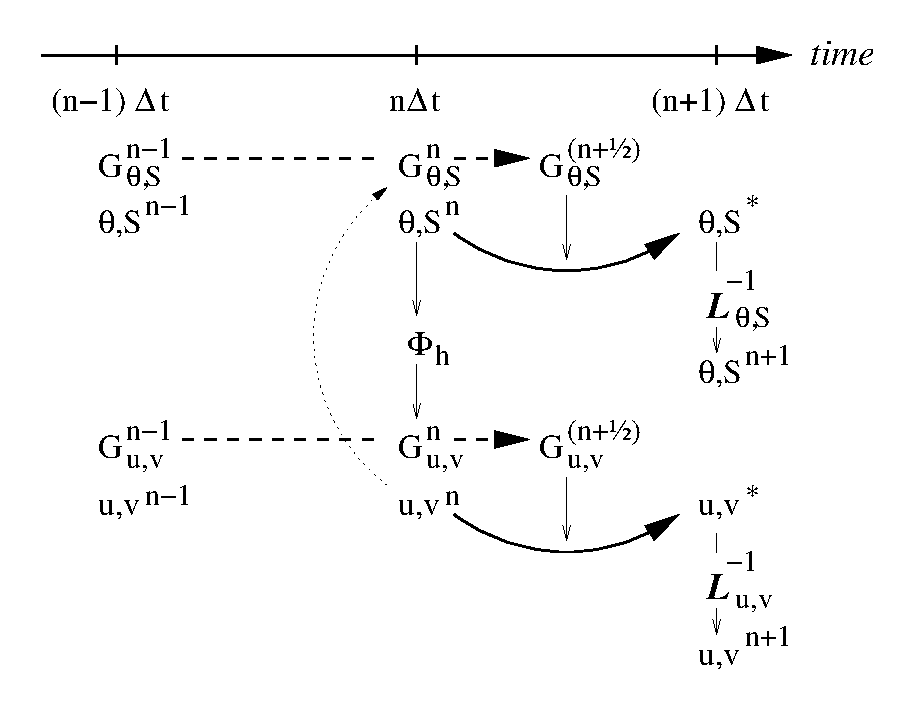
\includegraphics{part2/adams-bashforth-sync.eps}}
\end{center}
\caption{
A schematic of the explicit Adams-Bashforth and implicit time-stepping
phases of the algorithm. All prognostic variables are co-located in
time. Explicit tendancies are evaluated at time level $n$ as a
function of the state at that time level (dotted arrow). The explicit
tendancy from the previous time level, $n-1$, is used to extrapolate
tendancies to $n+1/2$ (dashed arrow). This extrapolated tendancy
allows variables to be stably integrated forward-in-time to render an
estimate ($*$-variables) at the $n+1$ time level (solid
arc-arrow). The operator ${\cal L}$ formed from implicit-in-time terms
is solved to yield the state variables at time level $n+1$. }
\label{fig:adams-bashforth-sync}
\end{figure}

\begin{figure}
\begin{center} \fbox{ \begin{minipage}{4.5in} \begin{tabbing}
aaa \= aaa \= aaa \= aaa \= aaa \= aaa \kill 
FORWARD\_STEP \\
\> THERMODYNAMICS \\
\>\> CALC\_GT \\
\>\>\> GAD\_CALC\_RHS \` $G_\theta^n = G_\theta( u, \theta^n )$ (\ref{eq:Gt-n-sync})\\
\>\>\> EXTERNAL\_FORCING \` $G_\theta^n = G_\theta^n + {\cal Q}$ \\
\>\>\> ADAMS\_BASHFORTH2 \` $G_\theta^{(n+1/2)}$ (\ref{eq:Gt-n+5-sync}) \\
\>\> TIMESTEP\_TRACER \` $\tau^*$ (\ref{eq:tstar-sync}) \\
\>\> IMPLDIFF \` $\tau^{(n+1)}$ (\ref{eq:t-n+1-sync}) \\
\> DYNAMICS \\
\>\> CALC\_PHI\_HYD \` $\phi_{hyd}^n$ (\ref{eq:phi-hyd-sync}) \\
\>\> MOM\_FLUXFORM or MOM\_VECINV \` $G_{\vec{\bf v}}^n$ (\ref{eq:Gv-n-sync})\\
\>\> TIMESTEP \` $\vec{\bf v}^*$ (\ref{eq:Gv-n+5-sync}, \ref{eq:vstar-sync}) \\
\>\> IMPLDIFF \` $\vec{\bf v}^{**}$ (\ref{eq:vstarstar-sync}) \\
\> SOLVE\_FOR\_PRESSURE \\
\>\> CALC\_DIV\_GHAT \` $\eta^*$ (\ref{eq:nstar-sync}) \\
\>\> CG2D \` $\eta^{n+1}$ (\ref{eq:elliptic-sync}) \\
\> THE\_CORRECTION\_STEP  \\
\>\> CALC\_GRAD\_PHI\_SURF \` $\nabla \eta^{n+1}$ \\
\>\> CORRECTION\_STEP \` $u^{n+1}$,$v^{n+1}$ (\ref{eq:v-n+1-sync})
\end{tabbing} \end{minipage} } \end{center}
\caption{
Calling tree for the overall synchronous algorithm using
Adams-Bashforth time-stepping.}
\label{fig:call-tree-adams-bashforth-sync}
\end{figure}

The Adams-Bashforth extrapolation of explicit tendancies fits neatly
into the pressure method algorithm when all state variables are
co-locacted in time. Fig.~\ref{fig:adams-bashforth-sync} illustrates
the location of variables in time and the evolution of the algorithm
with time. The algorithm can be represented by the sequential solution
of the follow equations:
\begin{eqnarray}
G_{\theta,S}^{n} & = & G_{\theta,S} ( u^n, \theta^n, S^n )
\label{eq:Gt-n-sync} \\
G_{\theta,S}^{(n+1/2)} & = & (3/2+\epsilon_{AB}) G_{\theta,S}^{n}-(1/2+\epsilon_{AB}) G_{\theta,S}^{n-1}
\label{eq:Gt-n+5-sync} \\
(\theta^*,S^*) & = & (\theta^{n},S^{n}) + \Delta t G_{\theta,S}^{(n+1/2)}
\label{eq:tstar-sync} \\
(\theta^{n+1},S^{n+1}) & = & {\cal L}^{-1}_{\theta,S} (\theta^*,S^*)
\label{eq:t-n+1-sync} \\
\phi^n_{hyd} & = & \int b(\theta^n,S^n) dr
\label{eq:phi-hyd-sync} \\
\vec{\bf G}_{\vec{\bf v}}^{n} & = & \vec{\bf G}_{\vec{\bf v}} ( \vec{\bf v}^n, \phi^n_{hyd} )
\label{eq:Gv-n-sync} \\
\vec{\bf G}_{\vec{\bf v}}^{(n+1/2)} & = & (3/2 + \epsilon_{AB} ) \vec{\bf G}_{\vec{\bf v}}^{n} - (1/2 + \epsilon_{AB} ) \vec{\bf G}_{\vec{\bf v}}^{n-1}
\label{eq:Gv-n+5-sync} \\
\vec{\bf v}^{*} & = & \vec{\bf v}^{n} + \Delta t \vec{\bf G}_{\vec{\bf v}}^{(n+1/2)}
\label{eq:vstar-sync} \\
\vec{\bf v}^{**} & = & {\cal L}_{\vec{\bf v}}^{-1} ( \vec{\bf v}^* )
\label{eq:vstarstar-sync} \\
\eta^* & = & \epsilon_{fs} \left( \eta^{n} +P-E+R \right)- \Delta t 
  \nabla \cdot H \widehat{ \vec{\bf v}^{**} }
\label{eq:nstar-sync} \\
\nabla \cdot g H \nabla \eta^{n+1} - \frac{\epsilon_{fs} \eta^{n+1}}{\Delta t^2}
& = & - \frac{\eta^*}{\Delta t^2}
\label{eq:elliptic-sync} \\
\vec{\bf v}^{n+1} & = & \vec{\bf v}^{*} - \Delta t g \nabla \eta^{n+1}
\label{eq:v-n+1-sync}
\end{eqnarray}
Fig.~\ref{fig:adams-bashforth-sync} illustrates the location of
variables in time and evolution of the algorithm with time. The
Adams-Bashforth extrapolation of the tracer tendancies is illustrated
byt the dashed arrow, the prediction at $n+1$ is indicated by the
solid arc. Inversion of the implicit terms, ${\cal
L}^{-1}_{\theta,S}$, then yields the new tracer fields at $n+1$. All
these operations are carried out in subroutine {\em THERMODYNAMICS} an
subsidiaries, which correspond to equations \ref{eq:Gt-n-sync} to
\ref{eq:t-n+1-sync}.
Similarly illustrated is the Adams-Bashforth extrapolation of
accelerations, stepping forward and solving of implicit viscosity and
surface pressure gradient terms, corresponding to equations
\ref{eq:Gv-n-sync} to \ref{eq:v-n+1-sync}.
These operations are carried out in subroutines {\em DYNAMCIS}, {\em
SOLVE\_FOR\_PRESSURE} and {\em THE\_CORRECTION\_STEP}. This, then,
represents an entire algorithm for stepping forward the model one
time-step. The corresponding calling tree is given in
\ref{fig:call-tree-adams-bashforth-sync}.

\section{Staggered baroclinic time-stepping}
\label{sect:adams-bashforth-staggered}

\begin{figure}
\begin{center}
\resizebox{5.5in}{!}{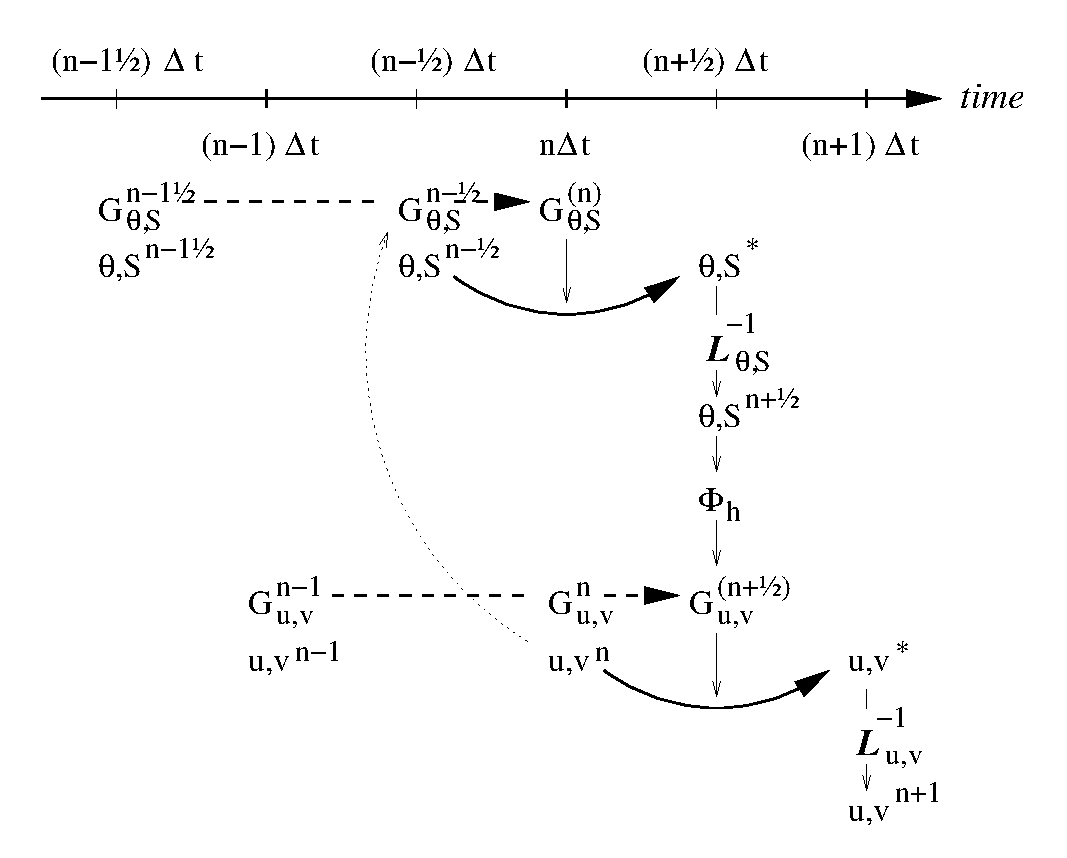
\includegraphics{part2/adams-bashforth-staggered.eps}}
\end{center}
\caption{
A schematic of the explicit Adams-Bashforth and implicit time-stepping
phases of the algorithm but with staggering in time of thermodynamic
variables with the flow. Explicit thermodynamics tendancies are
evaluated at time level $n-1/2$ as a function of the thermodynamics
state at that time level $n$ and flow at time $n$ (dotted arrow). The
explicit tendancy from the previous time level, $n-3/2$, is used to
extrapolate tendancies to $n$ (dashed arrow). This extrapolated
tendancy allows thermo-dynamics variables to be stably integrated
forward-in-time to render an estimate ($*$-variables) at the $n+1/2$
time level (solid arc-arrow). The implicit-in-time operator ${\cal
L_{\theta,S}}$ is solved to yield the thermodynamic variables at time
level $n+1/2$. These are then used to calculate the hydrostatic
pressure/geo-potential, $\phi_{hyd}$ (vertical arrows). The
hydrostatic pressure gradient is evaluated directly an time level
$n+1/2$ in stepping forward the flow variables from $n$ to $n+1$
(solid arc-arrow). }
\label{fig:adams-bashforth-staggered}
\end{figure}

For well stratified problems, internal gravity waves may be the
limiting process for determining a stable time-step. In the
circumstance, it is more efficient to stagger in time the
thermodynamic variables with the flow
variables. Fig.~\ref{fig:adams-bashforth-staggered} illustrates the
staggering and algorith. The key difference between this and
Fig.~\ref{fig:adams-bashforth-sync} is that the new thermodynamics
fields are used to compute the hydrostatic pressure at time level
$n+1/2$. The essentially allows the gravity wave terms to leap-frog in
time giving second order accuracy and more stability.

The essential change in the staggered algorithm is the calculation of
hydrostatic pressure which, in the context of the synchronous
algorithm involves replacing equation \ref{eq:phi-hyd-sync} with
\begin{displaymath}
\phi_{hyd}^n = \int b(\theta^{n+1},S^{n+1}) dr
\end{displaymath}
but the pressure gradient must also be taken out of the
Adams-Bashforth extrapoltion. Also, retaining the integer time-levels,
$n$ and $n+1$, does not give a user the sense of where variables are
located in time.  Instead, we re-write the entire algorithm,
\ref{eq:Gt-n-sync} to \ref{eq:v-n+1-sync}, annotating the
position in time of variables appropriately:
\begin{eqnarray}
G_{\theta,S}^{n-1/2} & = & G_{\theta,S} ( u^n, \theta^{n-1/2}, S^{n-1/2} )
\label{eq:Gt-n-staggered} \\
G_{\theta,S}^{(n)} & = & (3/2+\epsilon_{AB}) G_{\theta,S}^{n-1/2}-(1/2+\epsilon_{AB}) G_{\theta,S}^{n-3/2}
\label{eq:Gt-n+5-staggered} \\
(\theta^*,S^*) & = & (\theta^{n},S^{n}) + \Delta t G_{\theta,S}^{(n)}
\label{eq:tstar-staggered} \\
(\theta^{n+1/2},S^{n+1/2}) & = & {\cal L}^{-1}_{\theta,S} (\theta^*,S^*)
\label{eq:t-n+1-staggered} \\
\phi^{n+1/2}_{hyd} & = & \int b(\theta^{n+1/2},S^{n+1/2}) dr
\label{eq:phi-hyd-staggered} \\
\vec{\bf G}_{\vec{\bf v}}^{n} & = & \vec{\bf G}_{\vec{\bf v}} ( \vec{\bf v}^n )
\label{eq:Gv-n-staggered} \\
\vec{\bf G}_{\vec{\bf v}}^{(n+1/2)} & = & (3/2 + \epsilon_{AB} ) \vec{\bf G}_{\vec{\bf v}}^{n} - (1/2 + \epsilon_{AB} ) \vec{\bf G}_{\vec{\bf v}}^{n-1}
\label{eq:Gv-n+5-staggered} \\
\vec{\bf v}^{*} & = & \vec{\bf v}^{n} + \Delta t \left( \vec{\bf G}_{\vec{\bf v}}^{(n+1/2)} - \nabla \phi_{hyd}^{n+1/2} \right)
\label{eq:vstar-staggered} \\
\vec{\bf v}^{**} & = & {\cal L}_{\vec{\bf v}}^{-1} ( \vec{\bf v}^* )
\label{eq:vstarstar-staggered} \\
\eta^* & = & \epsilon_{fs} \left( \eta^{n} +P-E+R \right)- \Delta t 
  \nabla \cdot H \widehat{ \vec{\bf v}^{**} }
\label{eq:nstar-staggered} \\
\nabla \cdot g H \nabla \eta^{n+1} - \frac{\epsilon_{fs} \eta^{n+1}}{\Delta t^2}
& = & - \frac{\eta^*}{\Delta t^2}
\label{eq:elliptic-staggered} \\
\vec{\bf v}^{n+1} & = & \vec{\bf v}^{*} - \Delta t g \nabla \eta^{n+1}
\label{eq:v-n+1-staggered}
\end{eqnarray}
The calling sequence is unchanged from
Fig.~\ref{fig:call-tree-adams-bashforth-sync}. The staggered algorithm
is activated with the run-time flag {\bf staggerTimeStep=.TRUE.} in
{\em PARM01} of {\em data}.

The only difficulty with this approach is apparent in equation
$\ref{eq:Gt-n-staggered}$ and illustrated by the dotted arrow
connecting $u,v^n$ with $G_\theta^{n-1/2}$. The flow used to advect
tracers around is not naturally located in time. This could be avoided
by applying the Adams-Bashforth extrapolation to the tracer field
itself and advection that around but this is not yet available. We're
not aware of any detrimental effect of this feature. The difficulty
lies mainly in interpretation of what time-level variables and terms
correspond to.


\section{Non-hydrostatic formulation}
\label{sect:non-hydrostatic}

[to be written...]




\section{Variants on the Free Surface}

We now descibe the various formulations of the free-surface that
include non-linear forms, implicit in time using Crank-Nicholson,
explicit and [one day] split-explicit. First, we'll reiterate the
underlying algorithm but this time using the notation consistent with
the more general vertical coordinate $r$. The elliptic equation for
free-surface coordinate (units of $r$), correpsonding to
\ref{eq:discrete-time-backward-free-surface}, and
assuming no non-hydrostatic effects ($\epsilon_{nh} = 0$) is:
\begin{eqnarray}
\epsilon_{fs} {\eta}^{n+1} -
{\bf \nabla}_h \cdot \Delta t^2 (R_o-R_{fixed}) {\bf \nabla}_h b_s
{\eta}^{n+1} = {\eta}^*
\label{eq-solve2D}
\end{eqnarray}
where
\begin{eqnarray}
{\eta}^* = \epsilon_{fs} \: {\eta}^{n} -
\Delta t {\bf \nabla}_h \cdot \int_{R_{fixed}}^{R_o} \vec{\bf v}^* dr
\: + \: \epsilon_{fw} \Delta_t (P-E)^{n} 
\label{eq-solve2D_rhs}
\end{eqnarray}

\fbox{ \begin{minipage}{4.75in}
{\em S/R SOLVE\_FOR\_PRESSURE} ({\em solve\_for\_pressure.F})

$u^*$: {\bf GuNm1} ({\em DYNVARS.h})

$v^*$: {\bf GvNm1} ({\em DYNVARS.h})

$\eta^*$: {\bf cg2d\_b} (\em SOLVE\_FOR\_PRESSURE.h)

$\eta^{n+1}$: {\bf etaN} (\em DYNVARS.h)

\end{minipage} }


Once ${\eta}^{n+1}$ has been found, substituting into
\ref{eq-tDsC-Hmom} yields $\vec{\bf v}^{n+1}$ if the model is
hydrostatic ($\epsilon_{nh}=0$):
$$
\vec{\bf v}^{n+1} = \vec{\bf v}^{*}
- \Delta t {\bf \nabla}_h b_s {\eta}^{n+1}
$$

This is known as the correction step. However, when the model is
non-hydrostatic ($\epsilon_{nh}=1$) we need an additional step and an
additional equation for $\phi'_{nh}$. This is obtained by substituting
\ref{eq-tDsC-Hmom} and \ref{eq-tDsC-Vmom} into
\ref{eq-tDsC-cont}:
\begin{equation}
\left[ {\bf \nabla}_h^2 + \partial_{rr} \right] {\phi'_{nh}}^{n+1}
= \frac{1}{\Delta t} \left(
{\bf \nabla}_h \cdot \vec{\bf v}^{**} + \partial_r \dot{r}^* \right)
\end{equation}
where
\begin{displaymath}
\vec{\bf v}^{**} = \vec{\bf v}^* - \Delta t {\bf \nabla}_h b_s {\eta}^{n+1}
\end{displaymath}
Note that $\eta^{n+1}$ is also used to update the second RHS term
$\partial_r \dot{r}^* $ since
the vertical velocity at the surface ($\dot{r}_{surf}$) 
is evaluated as $(\eta^{n+1} - \eta^n) / \Delta t$.

Finally, the horizontal velocities at the new time level are found by:
\begin{equation}
\vec{\bf v}^{n+1} = \vec{\bf v}^{**}
- \epsilon_{nh} \Delta t {\bf \nabla}_h {\phi'_{nh}}^{n+1}
\end{equation}
and the vertical velocity is found by integrating the continuity
equation vertically.  Note that, for the convenience of the restart
procedure, the vertical integration of the continuity equation has
been moved to the beginning of the time step (instead of at the end),
without any consequence on the solution.

\fbox{ \begin{minipage}{4.75in}
{\em S/R CORRECTION\_STEP} ({\em correction\_step.F})

$\eta^{n+1}$: {\bf etaN} (\em DYNVARS.h)

$\phi_{nh}^{n+1}$: {\bf phi\_nh} (\em DYNVARS.h)

$u^*$: {\bf GuNm1} ({\em DYNVARS.h})

$v^*$: {\bf GvNm1} ({\em DYNVARS.h})

$u^{n+1}$: {\bf uVel} ({\em DYNVARS.h})

$v^{n+1}$: {\bf vVel} ({\em DYNVARS.h})

\end{minipage} }



Regarding the implementation of the surface pressure solver, all
computation are done within the routine {\it SOLVE\_FOR\_PRESSURE} and
its dependent calls.  The standard method to solve the 2D elliptic
problem (\ref{eq-solve2D}) uses the conjugate gradient method (routine
{\it CG2D}); the solver matrix and conjugate gradient operator are
only function of the discretized domain and are therefore evaluated
separately, before the time iteration loop, within {\it INI\_CG2D}.
The computation of the RHS $\eta^*$ is partly done in {\it
CALC\_DIV\_GHAT} and in {\it SOLVE\_FOR\_PRESSURE}.

The same method is applied for the non hydrostatic part, using a
conjugate gradient 3D solver ({\it CG3D}) that is initialized in {\it
INI\_CG3D}. The RHS terms of 2D and 3D problems are computed together
at the same point in the code.



\subsection{Crank-Nickelson barotropic time stepping}

The full implicit time stepping described previously is
unconditionally stable but damps the fast gravity waves, resulting in
a loss of potential energy.  The modification presented now allows one
to combine an implicit part ($\beta,\gamma$) and an explicit part
($1-\beta,1-\gamma$) for the surface pressure gradient ($\beta$) and
for the barotropic flow divergence ($\gamma$).
\\
For instance, $\beta=\gamma=1$ is the previous fully implicit scheme;
$\beta=\gamma=1/2$ is the non damping (energy conserving), unconditionally
stable, Crank-Nickelson scheme; $(\beta,\gamma)=(1,0)$ or $=(0,1)$
corresponds to the forward - backward scheme that conserves energy but is
only stable for small time steps.\\
In the code, $\beta,\gamma$ are defined as parameters, respectively 
{\it implicSurfPress}, {\it implicDiv2DFlow}. They are read from
the main data file "{\it data}" and are set by default to 1,1.

Equations \ref{eq-tDsC-Hmom} and \ref{eq-tDsC-eta} are modified as follows:
$$
\frac{ \vec{\bf v}^{n+1} }{ \Delta t }
+ {\bf \nabla}_h b_s [ \beta {\eta}^{n+1} + (1-\beta) {\eta}^{n} ] 
+ \epsilon_{nh} {\bf \nabla}_h {\phi'_{nh}}^{n+1}
 = \frac{ \vec{\bf v}^* }{ \Delta t }
$$
$$
\epsilon_{fs} \frac{ {\eta}^{n+1} - {\eta}^{n} }{ \Delta t}
+ {\bf \nabla}_h \cdot \int_{R_{fixed}}^{R_o} 
[ \gamma \vec{\bf v}^{n+1} + (1-\gamma) \vec{\bf v}^{n}] dr
= \epsilon_{fw} (P-E)
$$
where:
\begin{eqnarray*}
\vec{\bf v}^* & = &
\vec{\bf v} ^{n} + \Delta t \vec{\bf G}_{\vec{\bf v}} ^{(n+1/2)}
+ (\beta-1) \Delta t {\bf \nabla}_h b_s {\eta}^{n}
+ \Delta t {\bf \nabla}_h {\phi'_{hyd}}^{(n+1/2)}
\\
{\eta}^* & = &
\epsilon_{fs} {\eta}^{n} + \epsilon_{fw} \Delta t (P-E) 
- \Delta t {\bf \nabla}_h \cdot \int_{R_{fixed}}^{R_o} 
[ \gamma \vec{\bf v}^* + (1-\gamma) \vec{\bf v}^{n}] dr
\end{eqnarray*}
\\
In the hydrostatic case ($\epsilon_{nh}=0$), allowing us to find
${\eta}^{n+1}$, thus:
$$
\epsilon_{fs} {\eta}^{n+1} -
{\bf \nabla}_h \cdot \beta\gamma \Delta t^2 b_s (R_o - R_{fixed})
{\bf \nabla}_h {\eta}^{n+1}
= {\eta}^*
$$ 
and then to compute (correction step):
$$
\vec{\bf v}^{n+1} = \vec{\bf v}^{*}
- \beta \Delta t {\bf \nabla}_h b_s {\eta}^{n+1}
$$

The non-hydrostatic part is solved as described previously. 

Note that:
\begin{enumerate}
\item The non-hydrostatic part of the code has not yet been 
updated, so that this option cannot be used with $(\beta,\gamma) \neq (1,1)$.
\item The stability criteria with Crank-Nickelson time stepping
for the pure linear gravity wave problem in cartesian coordinates is:
\begin{itemize}
\item $\beta + \gamma < 1$ : unstable
\item $\beta \geq 1/2$ and $ \gamma \geq 1/2$ : stable
\item $\beta + \gamma \geq 1$ : stable if
$$ 
c_{max}^2 (\beta - 1/2)(\gamma - 1/2) + 1 \geq 0
$$
$$
\mbox{with }~
%c^2 = 2 g H {\Delta t}^2 
%(\frac{1-cos 2 \pi / k}{\Delta x^2} 
%+\frac{1-cos 2 \pi / l}{\Delta y^2})
%$$
%Practically, the most stringent condition is obtained with $k=l=2$ :
%$$
c_{max} =  2 \Delta t \: \sqrt{g H} \: 
\sqrt{ \frac{1}{\Delta x^2} + \frac{1}{\Delta y^2} }
$$
\end{itemize}
\end{enumerate}

